\section{\LaTeX 应用笔记}
本文档于\today 开始使用\LaTeX 作笔记文档。

\subsection{超链接应用}
超链接显示有2种:
\begin{itemize}
\item 链接和显示内容一致:\url{https://www.baidu.com}
\item 链接和显示内容不一致:\href{https://www.baidu.com}{百度链接}
\end{itemize}

\subsection{枚举项应用}
以下是枚举内容:
\begin{itemize}
\item 枚举1。
\item 枚举2。
\item 枚举3。
\item 枚举4。
\end{itemize}


\subsection{在正文中强调某个词语}
我要\emphasizebox{强abc调}这个词语。

\subsection{插入Linux命令}
\begin{commandbox}
 > sudo chsh -s zsh
\end{commandbox}

\subsection{用数字表示一个范围}
我要表示一个范围:$18\sim22$ 岁。

\subsection{插入一个Linux信息输出框}
\begin{messagebox}
On branch master
Your branch is ahead of 'origin/master' by 3 commits.
  (use "git push" to publish your local commits)
Changes not staged for commit:
  (use "git add <file>..." to update what will be committed)
  (use "git checkout -- <file>..." to discard changes in working directory)
\end{messagebox}

\subsection{测试codeout}
\begin{codeout}
codeout ccc
\end{codeout}


\subsection{基本代码块测试}
\begin{lstlisting}[language=C, numbers=left]
void main ()
{
    return;
}
\end{lstlisting}

\subsection{测试mycode}
\begin{myccode}[caption={hello工程}]
/* 这是一个hello工程 */
void main ()
{
    int cnt = 0;
    printf("Hello World: %d\n", cnt);
    return;
}
\end{myccode}

\subsection{空行分段 单个换行相当于空格}
老话说生活有五味,酸甜苦辣咸。苦是生命所不能避免的一味,叔本华说:“人生就是痛苦,我们可以把痛苦转换成幸福”,努力就是转化的过程,尽管在这个过程中,我们可能会感到更加辛苦。

苦,是人生的必经过程。人生就是一个“享受”痛苦和磨难的过程,这个过程是值得体会和拥有的。
人生本身就是一场与痛苦并存的旅行,并不像很多人想象的那么轻松,从生下来的那一天,我们就开始了人生的修行。

无论你生长在怎样的环
境中,你都会面临人生的各种难题。面对这些难题、困境,没有人可以不流泪流汗就轻轻松松地跨过去。经历得越多,越容易发现这个世界的真理——越怕吃苦,越有苦吃。那些心灵真正富足的人,其实都不怕吃苦。

\subsection{脚注命令}
苦\footnote{\emph 苦,是人生的必经过程。}

\subsection{引用}
\begin{quote}
老话说生活有五味,酸甜苦辣咸。
\end{quote}

\subsection{改变字体和字号}
\begin{quote}
\zihao{-5} \kaishu 老话说生活有五味,酸甜苦辣咸。
\end{quote}

\subsection{定理环境}
\begin{thm}[勾股定理]
一二三。
\end{thm}

\subsection{公式排版}
\begin{equation}
a(b+c) = ab + ac
\end{equation}

\begin{equation}
\angle ABC = \pi / 2
\end{equation}

\begin{equation}\label{eq:gougu}
AB^2 = BC^2 + AC^2
\end{equation}

\begin{equation}
90^\circ
\end{equation}

\subsection{插入图片}
%\begin{figure}[ht]
\begin{figure}[H]
\centering
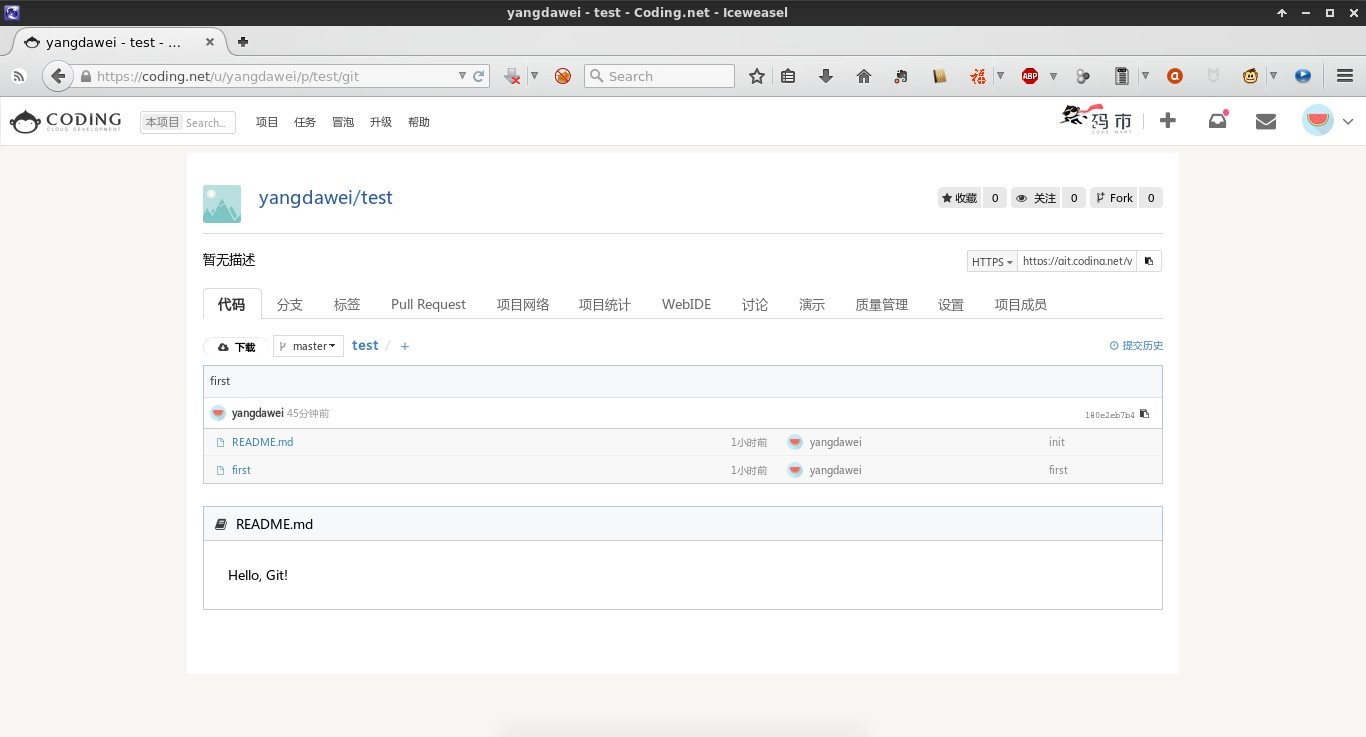
\includegraphics[height=5cm]{testcode.jpg}
\caption{建立项目}
\label{fig:createproject}
\end{figure}

\subsection{插入表格}
\begin{table}[H] %浮动环境
\begin{tabular}{|rrr|}
\hline
直角边 $a$ & 直角边 $b$ & 斜边 $c$ \\
\hline
3 & 4 & 5 \\  %分列
5 & 12 & 13 \\ %下一行
\hline
\end{tabular}
\end{table}

\subsection{引用公式和图表}
图 \ref{fig:createproject} 表示。

公式 \ref{eq:gougu} 方法。

另一种引用公式 \eqref{eq:gougu} 方法。 %添加\usepackage{amsmath}

\subsection{自定义新的命令}
使用newcommand命令。
符号度的新命令 $90\degree$ 。%注意:要加$$

\subsection{一些标点符号}
省略号\ldots \dots \# \quad \$ \quad \% \quad \& \quad \{ \quad \} \quad \_ \quad \textbackslash

中文标点使用全角输入,破折号shift+- ——,省略号shift+6……

忽略每行前面的空格,后面的空格多个当成一个,\TeX\ ing,\TeX{} ing. {\TeX} ing. 换行当空格I 
am Tex.汉字和字母自动添加空格tex。


